%!TEX root = rampMeteringJack.tex
\section{Modified 2x2 Piccoli model with Buffers}\label{sec:modified}
\subsection{Generalized mainline junction}
\frame{
  \setbeamercovered{transparent}
	\frametitle{Generalized mainline junction}
  \begin{itemize}
    \item<1-> Two incoming links
    \begin{itemize}
			\item Upstream mainline
			\item Onramp
		\end{itemize}
    \item<2-> Two outgoing links
    \begin{itemize}
			\item Downstream mainline
			\item Offramp
		\end{itemize}
 \end{itemize}
 
 \begin{figure}[ht]
	\centering
	{
	\resizebox{\columnwidth}{!}{
	

\begin{tikzpicture}[scale=1.4]

\def \linkWidth {1cm}
\def \nodeWidth {0.3cm}

\coordinate (arrow) at (1.8,0);
\coordinate (dots) at (0.5,0);
\coordinate (unit) at (2.5,0);

\node (link0) at (0,0) [rectangle, minimum width=\linkWidth, draw] {$0$};
\node (link1) at ($(link0) + 1*(unit)$) [rectangle, minimum width=\linkWidth, draw] {$1$};
\node (linkI) at ($(link1) + 2*(unit)$) [rectangle, minimum width=\linkWidth, draw] {$\icell$};
\node (nodeI) at ($(linkI) + 1*(unit)$) [circle, minimum width=\nodeWidth, draw] {$\icell$};

\node (onrampI) at ($(linkI)-(0,0.8)$) [rectangle, minimum width=\linkWidth, draw] {on-ramp $\icell$};
\node (offrampI) at ($(linkI) + 1.4*(unit) - (0,0.5)$) {};

\node (linkI1) at ($(nodeI) + 1.45*(unit)$) [rectangle, minimum width=\linkWidth, draw] {$\icell+1$};

\node (linkN) at ($(linkI1)+1.8*(unit)$) [rectangle, minimum width=\linkWidth, draw] {$\ncell$};

% link 0
\draw[->] ($(link0)-(arrow)$) -- (link0) node[above, midway] {$\inputflux{0}{\itime}$};
\draw[->] (link0) -- (link1) node[above, midway] {$\flowout{0}{\itime}$};

% link 1
\draw[->] (link1) -- ($(link1) + (arrow)$) node[above, midway] {$\flowout{1}{\itime}$};

%dots
\draw ($(link1) + (arrow) + (dots)$) node{$\dots$} ;

% link i
\draw[->] ($(linkI) - 1.3*(arrow)$) -- (linkI)node[above, xshift=-1.1cm] {$\flowin{\icell}{\itime}$};
\draw[->] (linkI) -- (nodeI) node[above, midway] {$\flowout{\icell}{\itime}$};
\draw[->] (nodeI) -- (linkI1) node[above, xshift=-1.1cm]{$\flowin{\icell+1}{\itime}$} ;

%node i
\draw[->] (onrampI) [anchor=right]-- (nodeI) node[below, midway]{$\rampflow{\icell}{\itime}$};
\draw[->] ($(onrampI) - (arrow)$) [anchor=right]-- (onrampI) node[above, midway]{$\inputflux{\icell}{\itime}$};
\draw[->] (nodeI) -- (offrampI) node[below, xshift=-0.3cm]{$\offrampratio{\icell}{\itime} \flowout{\icell}{\itime}$};

%link i+1
\draw[->] (linkI1) -- ($(linkI1) + (arrow)$) node[above, midway] {$\flowout{\icell+1}{\itime}$};

%dots
\draw ($(linkI1)+(arrow)+(dots)$) node{$\dots$} ;

% link N
\draw[->] ($(linkN) - (arrow)$) -- (linkN) node[above, midway] {$\flowin{\ncell}{\itime}$};
\draw[->] (linkN)--($(linkN) + (arrow)$) node[above, midway] {$\flowout{\ncell}{\itime}$};

% box
\draw[dashed] ($(linkI) + (-2,1)$) rectangle ($(nodeI) + (1.8,-1.5)$) node[below]{block $\icell$};

\end{tikzpicture}
}
	\caption{Mainline model with generalized $2\times 2$ junction.}
	\label{fig:system}}
 \end{figure}
 
 
}



\subsection{Conservation of demand at ramps}
\begin{frame}
	\frametitle{Weak boundary conditions}
  \begin{itemize}
    \item For continuous models, boundary conditions are typically specified as densities
    \begin{itemize}
			\item Theoretically, one can apply inverse flux map to obtain densities from flux demands.
		\end{itemize}
    \item Solved as $1 \times 1$ junctions.
    \item Boundary condition \textbf{DOES NOT} always apply (see Figure~\ref{fig:weakBCShock}). Information from this time step is ``lost''. OK for estimation, but demand not satisfied for control schemes.
 \end{itemize}
 
 \begin{columns}
	\column{0.5 \textwidth}
	\begin{figure}[ht]
\centering
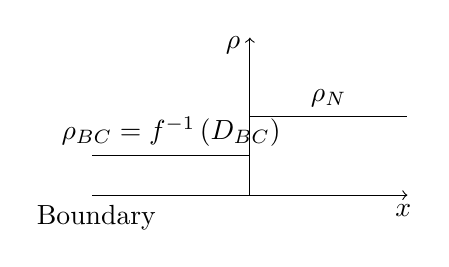
\begin{tikzpicture}[scale=0.5]
\draw [<-] (0,4) -- (0,0);
\draw [->] (-4,0) -- (4,0);
\draw (0,1)--(-4,1);
\draw (0,2)--(4,2);
\node [below] at (3.9,0) {$x$};
\node [below] at (-3.9,0) {Boundary};
\node [above] at (-2,1) {$\rho_{BC}=f^{-1}\left( D_{BC} \right)$};
\node [above] at (2,2) {$\rho_{N}$};
\node [left] at (0,3.8) {$\rho$};
\end{tikzpicture}
\caption{Riemann problem at boundary with low boundary density $\rho_{BC}$ and high network density $\rho_{N}$.}
\label{fig:weakBCDensities}
\end{figure}
	\pause
	\column{0.5 \textwidth}
	\begin{figure}[ht]
\centering
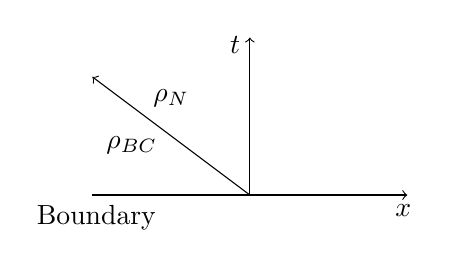
\begin{tikzpicture}[scale=0.5]
\draw [<-] (0,4) -- (0,0);
\draw [->] (-4,0) -- (4,0);
\draw[->] (0,0)--(-4,3);
\node [below] at (3.9,0) {$x$};
\node [below] at (-3.9,0) {Boundary};
\node [above] at (-3,0.8) {$\rho_{BC}$};
\node [above] at (-2,2) {$\rho_{N}$};
\node [left] at (0,3.8) {$t$};
\end{tikzpicture}
\caption{Boundary density condition does not enter network due to congestion.}
\label{fig:weakBCShock}
\end{figure}
	\end{columns}
\end{frame}

\global\long\def\actualrampflowsymbol{D}
\global\long\def\actualrampflow#1#2{\actualrampflowsymbol_{#1}\left(#2\right)}
\global\long\def\totalrampflowsymbol{\bar{D}}
\global\long\def\totalrampflow#1#2{\totalrampflowsymbol_{#1}\left(#2\right)}
\global\long\def\fluxsymbol{\gamma}
\global\long\def\flux#1#2{\fluxsymbol_{#1}\left(#2\right)}
\global\long\def\rampfluxsymbol{\gamma^{\text{r}}}
\global\long\def\rampflux#1#2{\rampfluxsymbol_{#1}\left(#2\right)}
\global\long\def\maxrampfluxsymbol{\gamma^{\text{r,\ensuremath{\max}}}}
\global\long\def\maxrampflux#1{\gamma_{#1}^{\text{r,\ensuremath{\max}}}}


\begin{frame}

\frametitle{Solution to demand conservation: Buffers}
Introduce a point queue buffer, $d\rampqueue{\icell}t$, for cell $i$ at time $t$ as the model for onramps:
\begin{equation}
\frac{d\rampqueue{\icell}t}{dt} = \totalrampflow{\icell}t- r_{i}\left( t \right) \label{eq:rampode} 
\end{equation}
where the ramp's demand at the junction is given by:
\begin{equation}
\rampdemand{\icell}t = \begin{cases}
r_{i}^{\max} & \rampqueue{\icell}t>0\\
\min \left( r_{i}^{\max} , \totalrampflow{\icell}t \right) & \text{otherwise}
\end{cases}
\end{equation}

\begin{fact}
Ramp demand is now conserved by definition
\end{fact}

\end{frame}


\subsection{Max junction flux and ramp-metering model}
\begin{frame}

	\frametitle{Maximizing junction flux blocks onramp}
	\begin{itemize}
		\item<1-> Using standard Piccoli model, $2 \times 2$ junctions permit a unique solution \textbf{without} priorities.
		\item<2-> Since turning ratio from onramp to offramp is $0$, mainline flux will reach capacity before onramp flux allowed. See Figure~\ref{fig:bad2by2}
		\item<3-> \textbf{Poor model of reality, where physical priorities still exist}
	\end{itemize}

 \begin{figure}[ht]
	\centering
	{
	\resizebox{.5 \columnwidth}{!}{
	\input{bad2by2Tikz}}
	\caption{Flux maximization across junction blocks flux from onramp.}
	\label{fig:bad2by2}}
 \end{figure}

\end{frame}

\begin{frame}

	\frametitle{Solution: Maximize flux into downstream mainline}
	Instead of maximizing total flux across junction, $J = f_i + r_i$, we instead maximize the flux into just the downstream mainline,
	\begin{equation}
	J' = \left(1 - \beta \right) f_i + r_i
	\end{equation}
	This makes the supply line and objective lines parallel, thus necessitating the reintroduction of a priority parameter, $P$.

	\textbf{Note:} The same could be accomplished with a multi-objective cost function that maximizes total flux while penalizing deviations from priority.
	
 \begin{figure}[ht]
	\centering
	{
	\resizebox{.4 \columnwidth}{!}{
	\tikzset{dashdot/.style={dash pattern=on 2pt off 3pt on 4pt off 3pt}}

\begin{tikzpicture}[domain=0:1]

\def \rampDem{2}
\def \dem{2.5}
\def \priorityRat{0.7}
\def \splitRat{0.4}
\def \totalFlow{2.1}

\coordinate (Z) at (0,0);
\coordinate (I1) at (\rampDem, 0);
\coordinate (I2) at (0, \dem);
\coordinate (I3) at (\rampDem, \dem);
\coordinate (A) at (0, {\totalFlow/(1-\splitRat)});
\coordinate (B) at (\totalFlow, 0);
\coordinate (C) at ({(1-\priorityRat)/\priorityRat*\dem}, \dem);
\coordinate (Top) at (3,3);
\coordinate (P) at (intersection of A--B and Z--Top);


\draw[->] (Z) -- (3.5,0) node[below right]{$\rampflow{\icell}{\itime}$};
\draw[->] (Z) -- (0,4) node[left]{$\flowout{\icell}{\itime}$};
\draw[->] (Z) -- (Top) node[right]{$P$};
\draw[dashed] (I3) -- (I1) node[below]{$\rampdemand{\icell}{\itime}$};
\draw[dashed] (I3) -- (I2) node[left]{$\celldemand{\icell}{\itime}$};
\draw[color=red, radius=.1] (P) circle;
\draw[dashdot, ultra thick, color=green] (A) -- (B) node [xshift=3cm, yshift=2cm]{$\left(1 - \beta \right)\flowout{\icell}{\itime} + \rampflow{\icell}{\itime} = const$};

\end{tikzpicture}}
	\caption{Reintroduction of priority vector to ``unblock'' ramp flux.}
	\label{fig:good2by2}}
 \end{figure}

\end{frame}

